\documentclass[aspectratio=1610, professionalfonts, 13pt]{beamer}

% Lade das TU Dortund Theme von Max Nöthe
\usefonttheme[onlymath]{serif}
\usetheme[showtotalframes]{tudo}

% Lade richtiges Sprachpaket
\ifluatex
    \usepackage{polyglossia}
    \setmainlanguage{english}
\else
    \ifxetex
        \usepackage{polyglossia}
        \setmainlanguage{german}
    \else
        \usepackage[german]{babel}
    \fi
\fi

% Lade wichtige Mathematikpakete
\usepackage{amsmath}
\usepackage{amssymb}
\usepackage{mathtools}
\usepackage{cancel}
\usepackage[
  locale=DE,                   % deutsche Einstellungen
  separate-uncertainty=true,   % Immer Fehler mit \pm
  per-mode=symbol-or-fraction, % m/s im Text, sonst Brüche
]{siunitx}
\usepackage[absolute,overlay]{textpos}
\usepackage{framed}
\usepackage{multicol}
\usepackage{setspace}
\usepackage{graphicx}
\usepackage{booktabs}
\usepackage{caption}
\usepackage{appendixnumberbeamer}
\usepackage{tikz}
\usepackage[export]{adjustbox}
\usepackage{color}
\usepackage{animate}


% Lade Paket zur Nutzung von Schleifen
\usepackage{forloop}

% ------------------------- Präsentationsinformationen -------------------------

% Titel:
\title{\textbf{Analysis Of The Crab Nebula Using FACT's Photon Stream Data}}
% Autoren:
\author[K.\ Sedlaczek]{\textit{Kevin Sedlaczek}, Maximilian Nöthe for the FACT-Collaboration}


% Datum:
\date{20. March 2018}
\date[20. March 2018]{DPG-Frühjahrstagung 2018 Würzburg}
% Lehrstuhl/Fakultät:
\institute[TU Dortmund]{Lehrstuhl für Experimentelle Physik 5}

\institute[%
  {
\includegraphics[height=\headerheight]{logos/fact.pdf}}%
  \hspace{1em}%
  {
\includegraphics[height=\headerheight]{logos/e5logo.pdf}}%
]{
  {
\includegraphics[height=0.75cm]{logos/tu.pdf}}%
  \hspace{1em}%
  {
\includegraphics[height=0.75cm]{logos/ethz.pdf}}%
  \hspace{1em}%
  {
\includegraphics[height=0.75cm]{logos/isdc.pdf}}%
  \hspace{1em}%
  {
\includegraphics[height=0.75cm]{logos/uniwue.pdf}}%
}

% Titelgrafik:
% \titlegraphic{
\includegraphics[width=0.4\textwidth]{logos/FACTLogo_preliminary.png}\hfill
\includegraphics[width=0.4\textwidth]{logos/e5logo_green_text.pdf}}


\begin{document}

\maketitle

\section{The First G-APD Cherenkov Telescope}

\begin{frame}[t]{The First G-APD Cherenkov Telescope}
  \begin{multicols}{2}
    \vspace*{\fill}
    \begin{figure}
        \centering
        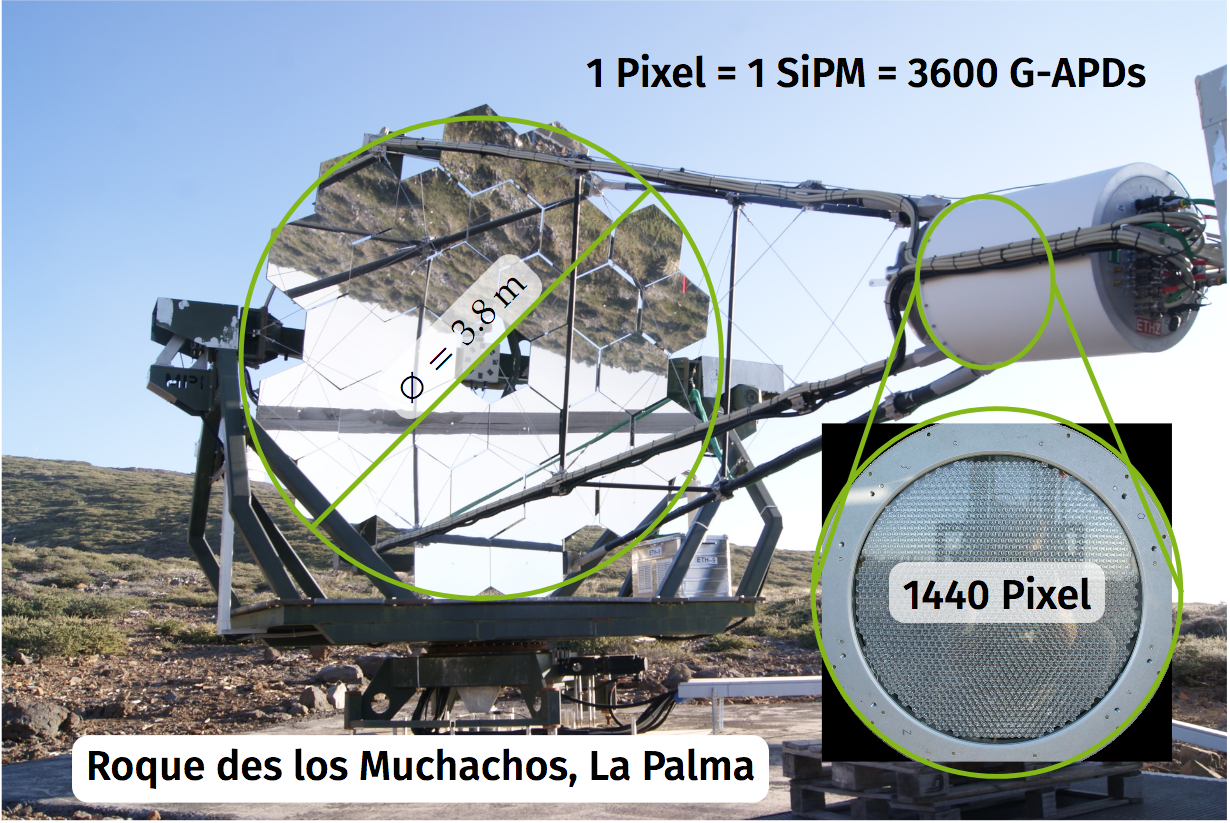
\includegraphics[width=0.5\textwidth]{fig/fact.png}
    \end{figure}
    \columnbreak
    \vspace*{\fill}
      \begin{itemize}
        \item located on Roque des los Muchachos, La Palma
        \item build to demonstrate novel light sensors \textit{silicon photo multipliers} (SiPM)
        \item offer possibility to operate under much brighter light conditions
        \item camera has single photon resolution
    \end{itemize}
    \vspace*{\fill}
  \end{multicols}
\end{frame}

\section{The Photon Stream Data}

\begin{frame}[t]{The Photon Stream Data}
    \large{\textbf{Rationale:}}
    \begin{itemize}
        \item FACT records data in format close to readout hardware
        \item raw data tedious to do physics analysis with: physics format required! \\ $\rightarrow$ \textbf{Photon Stream}
        \item superposition of multiple photon signals
        \item reconstruct arrival time of single photons by subtraction their pulse shapes
        \item list of lists of arrival times 
        \item smaller file size: possible to compress all FACT data to fit on one 10TB drive 
        \item simplify \textit{exchange} and \textit{analysis}, gain timing knowledge
        \item do physics analysis on an SiPM based IACT
    \end{itemize}
\end{frame}

\begin{frame}[t]{The Photon Stream Data}
    \begin{figure}
        \centering
        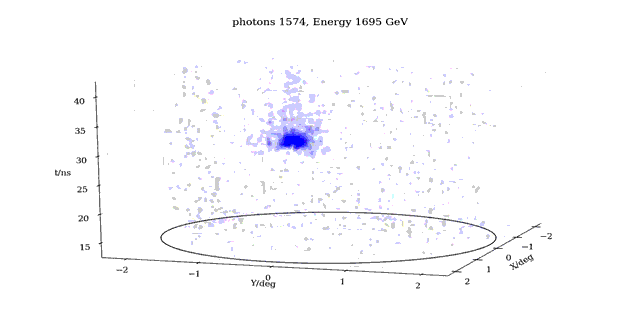
\includegraphics[width=0.75\textwidth]{fig/event/example_event_small-15.png}
        \caption{Represent \textbf{I}maging \textbf{A}tmospheric \textbf{C}herenkov \textbf{T}elescope events using single photons}
    \end{figure}
\end{frame}

\section{The Data Set: Crab Nebula}

\begin{frame}[t]{The Crab Nebula}
  \begin{multicols}{2}
    \begin{figure}
        \centering
        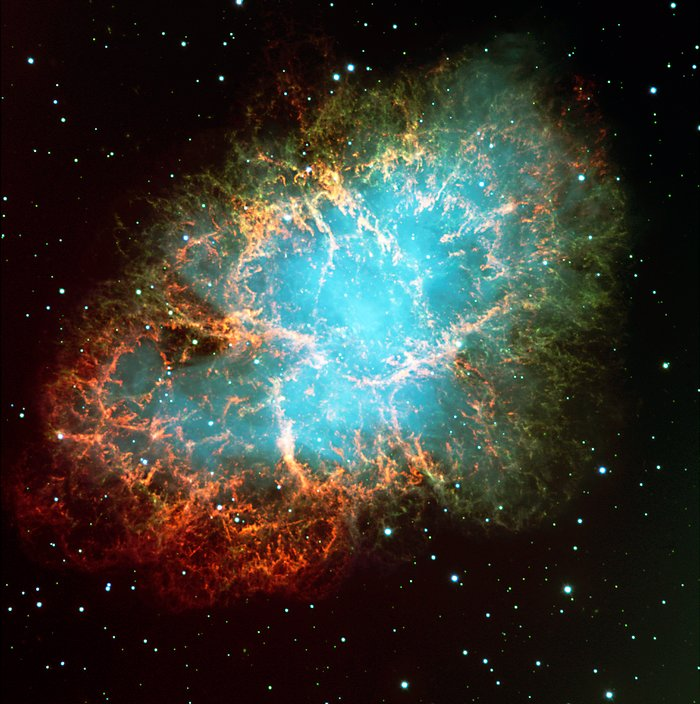
\includegraphics[width=0.4\textwidth]{fig/crab.jpg}
    \end{figure}
    \columnbreak
    \vspace*{\fill}
    \begin{itemize}
        \item remnant of super nova explosion
        \item distance is about $6000\,\text{ly}$
        \item neutron star at the centre of cloud
    \end{itemize}
    \vspace*{\fill}
  \end{multicols}
\end{frame}

\section{The Data Set: FACT open data crab sample}

\begin{frame}[t]{The Data set: FACT open data crab sample}
    \begin{multicols}{2}
        \begin{figure}
            \centering
            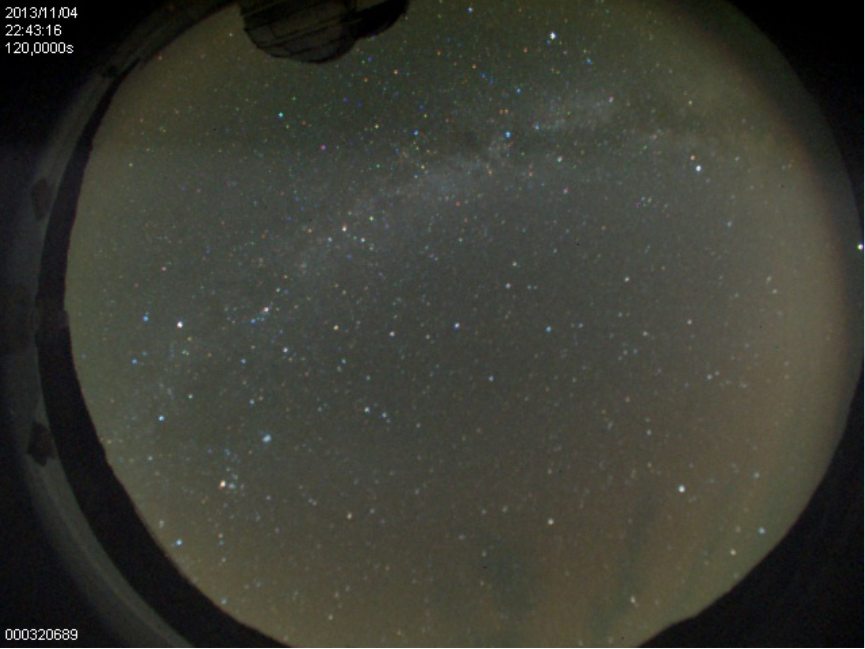
\includegraphics[width=0.4\textwidth]{fig/cond.png}
        \end{figure}
    \columnbreak
    \vspace*{\fill}
        \begin{itemize}
            \item \url{https://fact-project.org/data}
            \item Crab Nebula observations from November 2013
            \item including gamma-ray and proton simulations
            \item $17.7$ hours of observations
        \end{itemize}
    \vspace*{\fill}
  \end{multicols}
\end{frame}

\section{The Analysis}

\begin{frame}[t]{The Analysis}
    \begin{itemize}
        \item \textbf{{\color{tugreen} aim}}: test the Photon Stream data in a physics analysis
        \item \textbf{{\color{tugreen} Crab Nebula}}: well measured source of cosmic gamma rays $\rightarrow$ comparative analysis 
    \end{itemize}
FACT Analysis chain:
    \begin{enumerate}
        \item calibration of data
        \item image cleaning $\rightarrow$ pure shower image remains
    \end{enumerate}
\textbf{{\color{tugreen} This Analysis}} so far:
    \begin{enumerate}\addtocounter{enumi}{2}
        \item Parametrization: calculate useful parameters
        \item distinguish protons (background) from gammas
        \item reconstruct direction and energy of particles
    \end{enumerate}
\end{frame}

\begin{frame}[t]{Parameterization}
    \begin{multicols}{2}
        \begin{figure}
            \centering
            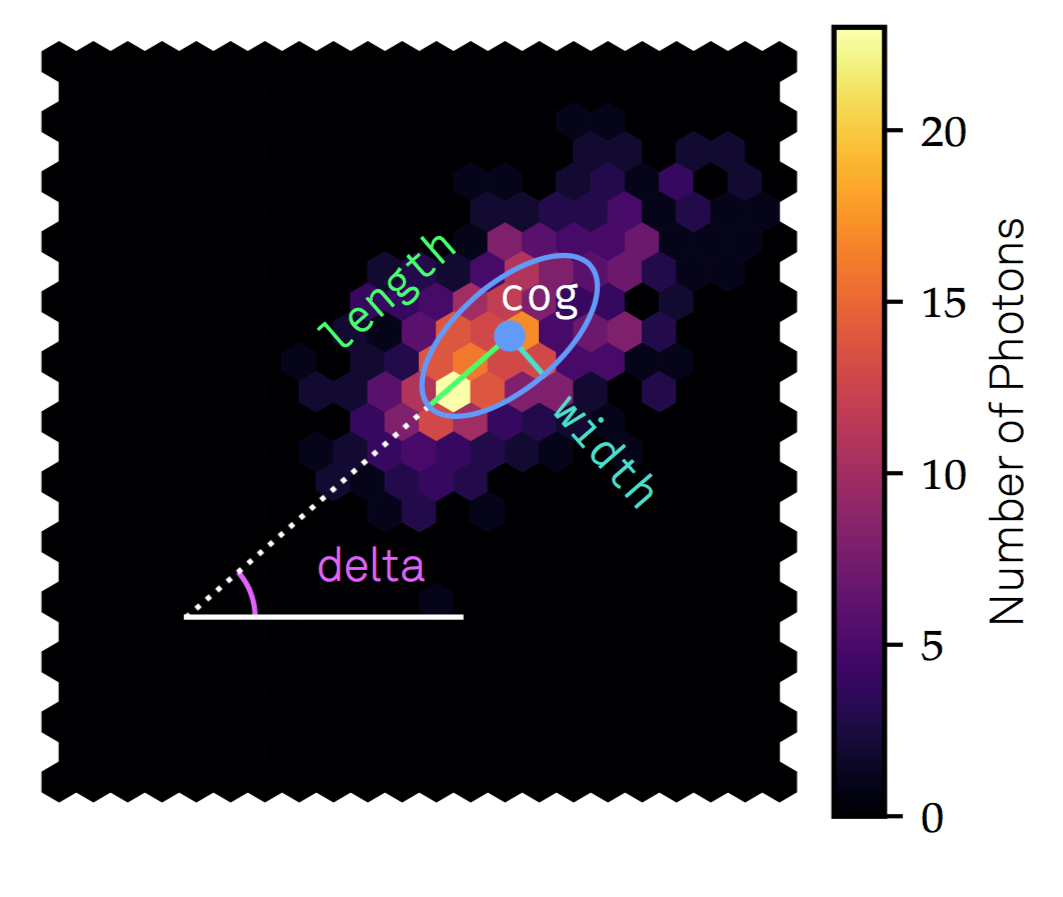
\includegraphics[width=0.5\textwidth]{fig/hillas.png}
        \end{figure}
    \columnbreak
Hillas parameters:
    \begin{itemize}
        \item \textbf{{\color{tugreen} size}}: number of photons in cluster
        \item \textbf{{\color{tugreen} length}}: std. dev. along long half-axis
        \item \textbf{{\color{tugreen} width}}: std. dev. along short half-axis
        \item \textbf{{\color{tugreen} delta}}: angle between length and disp
    \end{itemize}
    \end{multicols}
\end{frame}

\begin{frame}[t]{Parameterization}
    \begin{multicols}{2}
        \begin{figure}
            \centering
            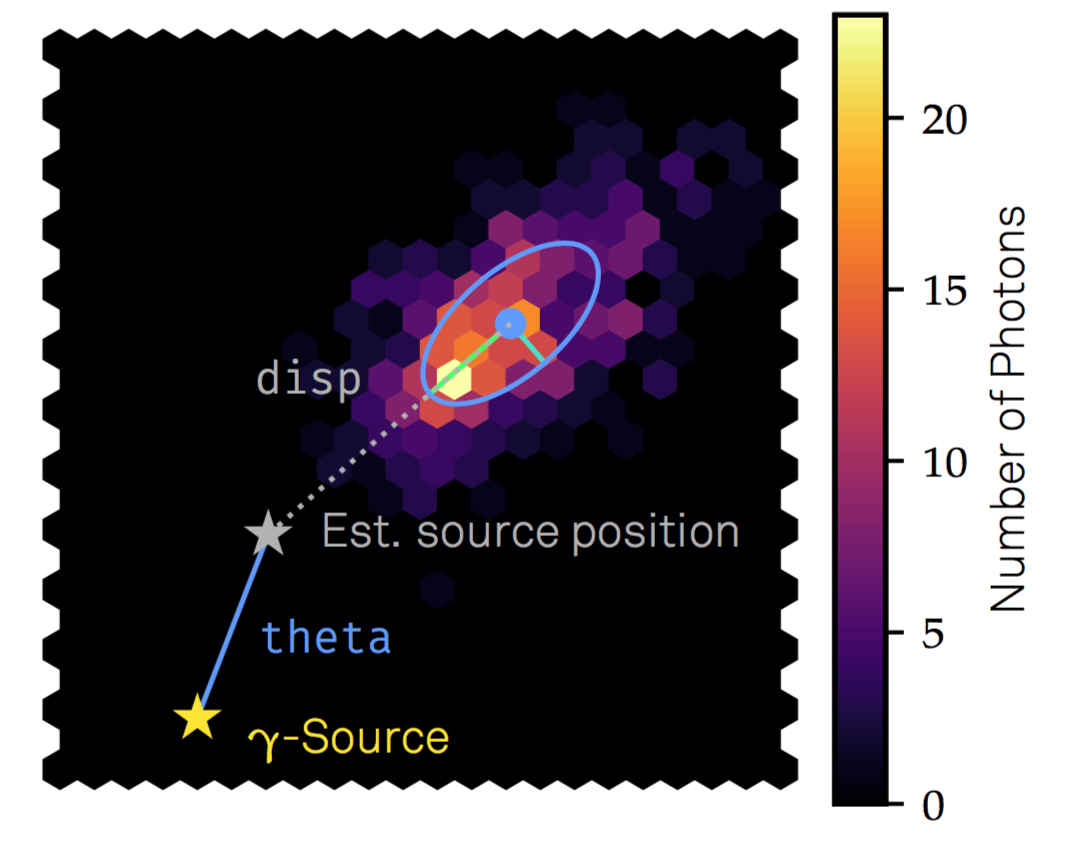
\includegraphics[width=0.5\textwidth]{fig/disp.png}
        \end{figure}
    \columnbreak
Source position reconstruction via disp-method:
    \begin{itemize}
        \item \textbf{{\color{tugreen} |disp|}}: distance from centre of gravity to target
        \item \textbf{{\color{tugreen} sgn(disp)}}: Head\/Tail-Disambiguation
        \item \textbf{{\color{tugreen} theta}}: distance between reconstructed and true origin
    \end{itemize}
    \end{multicols}
\end{frame}

\begin{frame}[t]{Tools}
Machine learning with FACT classifier-tools \url{https://github.com/fact-project/classifier-tools} \\
\textbf{{\color{tugreen} Energy estimation}}:
\begin{itemize}
    \item regressor: \texttt{klaas\_energy\_regressor}
\end{itemize}
\textbf{{\color{tugreen} Gamma-hadron-separation}}:
\begin{itemize}
    \item classification: \texttt{klaas\_separation\_model}
\end{itemize}
\textbf{{\color{tugreen} Origin reconstruction}}:
\begin{itemize}
    \item two step task: regression of |disp| and classification of sgn(disp)
    \item regression and classification: \texttt{klaas\_disp\_regressor}
\end{itemize}
\end{frame}

\section{results}

\begin{frame}[t]{Results}
\textbf{{\color{tugreen} Energy estimation}}:
\begin{itemize}
    \item 5 fold cross validation
    % \item Cross validated $\text{R}^2$ scores: $[ 0.59063531  0.60790374  0.6160266   0.61456317  0.60328615]$
    \item Mean $\text{R}^2$ score from CV: $0.6065\,\pm\,0.0092$
\end{itemize}
\textbf{{\color{tugreen} Separation}}:
\begin{itemize}
    \item 5 fold cross validation
    \item training on $100\,000$ signal and background events
    \item mean AUC ROC: $0.8104$
\end{itemize}
\textbf{{\color{tugreen} Origin reconstruction}}:
\begin{itemize}
    \item 5 fold cross validation
    \item training on $100000$ gamma and proton events
    \item mean AUC ROC: $0.8114$
\end{itemize}
\end{frame}

\section{outlook}

\begin{frame}[t]{Outlook}
\begin{itemize}
    \item test
    \item test
\end{itemize}
\end{frame}


%-------------------------------------------------------------------------------
\section{Back up}
%-------------------------------------------------------------------------------
\appendix

\begin{frame}[t]{}
  \centering
  \textcolor{tugreen}{\Huge{Back Up}}
\end{frame}

\end{document}
